\documentclass[aspectratio=169]{beamer}
\mode<presentation>{
    \usetheme{Frankfurt}
    \usecolortheme{rose}}
%%%%%%%%%%%%%%%%%%%%%%%%%%%%%%%%%%%%%%%%%%%%%%%%%%
\usepackage[utf8]{inputenc}
\usepackage[english]{babel}
\usepackage{graphicx} 
\usepackage{booktabs}
\usepackage{subcaption}
\usepackage{multirow}
\usepackage{xcolor}
\usepackage{amsthm}
\usepackage{amssymb}
\usepackage{amsmath}    
\usepackage{listings}
\usepackage{longtable}
\usepackage{lscape}
\usepackage[T1]{fontenc}
\usepackage{txfonts}
\usepackage{ragged2e}
\usepackage{etoolbox}
\usepackage{hyperref}   
\usepackage{transparent}
\usepackage{epstopdf}
\usepackage{enumerate}
\usepackage{multicol}
\usepackage{ragged2e}
%%%%%%%%%%%%%%%%%%%%%%%%%%%%%%%%%%%%%%%%%%%%%%%%%%
\newcommand{\Vv}{\overline{v}}%Letra v de solução
\newcommand{\Ww}{\overline{w}}%Letra w de solução
\newcommand{\kk}{\kappa}%Letra kappa
\newcommand{\cc}{\lambda}%Letra lambda
\newcommand{\ct}{\widetilde{C}}%Letra c com tiu
\newcommand{\zz}{{\mathbf{z}}}%Letra z de campo vetorial
\newcommand{\vv}{\nu}%Letra nu
\newcommand{\pp}{\widetilde{p}}%Letra p com acento
\newcommand{\pc}{p^{*}}%Letra p conjugada
\newcommand{\dd}{{\hspace*{0.08cm}}{\mathrm{d}}}%Letra p conjugada
\newcommand{\MM}{{\mathcal{M}}}%Letra p conjugada
\newcommand{\IN}{{\scriptscriptstyle{N}}}%Letra p conjugada
% CONJUNTOS E ESPAÇOS
\newcommand{\DMIO}{{\mathcal{DM}}^\infty(\Omega)}
\newcommand{\BVo}{{BV}(\Omega)}%Espaço BV de Omega
\newcommand{\IBV}{_{\scriptscriptstyle{BV}}}%Indice BV
\newcommand{\BVloc}{{BV}_{loc}(\Omega)}%Espaço BV de Omega
\newcommand{\LpO}{{L}^p(\Omega)}%Espaço L p de Omega
\newcommand{\ILp}{_{\scriptscriptstyle{L}^p}}%Indice L p 
\newcommand{\Linfo}{\emph{L}^\infty(\Omega)}%L infinito de Omega
\newcommand{\Linforn}{{L}^\infty(\Omega,{\mathbb{R}}^N)}%L infitiro de Omega em Rn
\newcommand{\ILinf}{_{\scriptscriptstyle{{L}}^\infty}}%L infitiro de Omega em Rn
\newcommand{\LUmO}{{\emph{L}}^1(\Omega)}%Espaço L 1 de Omega
\newcommand{\ILUmO}{_{\scriptscriptstyle{\emph{L}}^1(\Omega)}}%Indice L 1 de Omega
\newcommand{\ILUm}{_{\scriptscriptstyle{L}^1}}%Indice L 1 de Omega
\newcommand{\Diso}{{\mathcal{D}}^\prime(\Omega)}%Espaço das distribuições em Omega 
\newcommand{\IDis}{_{\scriptscriptstyle{\mathcal{D}}^\prime}}%Espaço das distribuições em Omega
\newcommand{\WumpzO}{{W}^{1,p}_0(\Omega)}%Espaço das W 1 p 0 de Omega
\newcommand{\IWumpz}{_{\scriptscriptstyle{W}^{1,p}_0} }%Indice do espaço das W 1 p 0
\newcommand{\WumpO}{{W}^{1,p}(\Omega)}%Espaço das W 1 p de Omega
\newcommand{\CUmCO}{{\mathcal{C}}^{1}_0(\Omega)}%Espaço C Um com suporte Compacto em Omega
\newcommand{\ICUmC}{_{\scriptscriptstyle{\mathcal{C}}^{1}_0}}%Espaço C Um com suporte Compacto em Omega
\newcommand{\CInfZO}{{\mathcal{C}}^{\infty}_0(\Omega)}% EspaçoC infinito de 0 em Omega
\newcommand{\CInfCO}{{\mathcal{C}}^{\infty}_0(\Omega)}% EspaçoC infinito de 0 em Omega
\newcommand{\CInfO}{{\mathcal{C}}^{\infty}(\Omega)}% EspaçoC infinito em Omega
\newcommand{\CO}{{\mathcal{C}}(\Omega)}
\newcommand{\ICInfZ}{_{\scriptscriptstyle{\mathcal{C}}^{\infty}_0}}% Indice C infinito de 0
\newcommand{\Cc}{{\mathbb{C}}}%Conjunto dos complexos
\newcommand{\Rr}{{\mathbb{R}}}%Conjunto dos Reais
\newcommand{\Nn}{{\mathbb{N}}}%Conjunto dos naturais
\newcommand{\DDo}{{\mathcal{D}}(\Omega)}%Espaço das funções testes
% OPERADORES
\newcommand{\sign}{{\text{sign}}}%Operador sign   
\newcommand{\dive}{{\text{div}}}%Operador divergente
\newcommand{\umlapla}{\text{div}\left(\dfrac{Du}{\left|Du\right| } \right)}%aOperador 1-laplaciano
\newcommand{\IntO}{\displaystyle\int_\Omega}%Integral sobre omega
\newcommand{\IntFO}{\displaystyle\int_{\partial\Omega}}%Integral sobre a fronteira de omega
\newcommand{\IntZS}{\displaystyle\int_{0}^s}%Integral de 0 a s
\newcommand{\IntSzS}{\displaystyle\int_{s_0}^s}%Integral de s_0 a s
\newcommand{\IntZSz}{\displaystyle\int_{0}^{s_0}}%Integral de 0 a s_0
\newcommand{\MedH}{{\mathcal{H}}^{N-1}}%Medida de Hausdorf de N-1
\newcommand{\Deln}{\Delta}
\newcommand{\Deli}{\nabla}
\newcommand{\ComO}{\left|\Omega\right| }
\newcommand{\supp}{{\text{supp}}}%Operador suporte

\newcommand{\liminfpum}{{\liminf\limits_{p\to 1^+}}}
\newcommand{\limsuppum}{{\limsup\limits_{p\to 1^+}}}
\newcommand{\limsups}{{\limsup\limits_{s\to 0}}}
\newcommand{\Impli}{\Rightarrow}
\newcommand{\Vai}{\longrightarrow}
\newcommand{\Chega}{\longmapsto}
\newcommand{\ToFr}{\rightharpoonup}


\newcommand{\Moe}{\left|}
\newcommand{\Mod}{\right|}
\newcommand{\Noe}{\left\|}
\newcommand{\Nod}{\right\|}
\newcommand{\NBVe}{\left|\hspace*{-0.05cm}\left|\hspace*{-0.05cm}\left|}
\newcommand{\NBVd}{\right|\hspace*{-0.05cm}\right|\hspace*{-0.05cm}\right|\IBV}
\newcommand{\Pae}{\left( }
\newcommand{\Pad}{\right) }
\newcommand{\Poe}{\left\langle}
\newcommand{\Pod}{\right\rangle}
\newcommand{\Que}{\left[}
\newcommand{\Qud}{\right] }

\setbeamertemplate{theorems}[ams style]
%\theoremstyle{Definition}
\newtheorem{ter}{Teorema}
\newtheorem{terr}{Teorema}
\newtheorem{defin}{Definição}
\newtheorem{lema}{Lema}
\newtheorem{obs}{Observação}
\newtheorem{prop}{Proposição}
\newtheorem{exem}{Exemplo}
%%%%%%%%%%%%%%%%%%%%%%%%%%%%%%%%%%%%%%%%%%%%%%%%%%
% Placeholder image to prevent compilation error. Replace with \includegraphics when needed.
\titlegraphic{
    \begin{center}
        
\includegraphics[width=3.5cm]{pic/AVVR03.eps}
    \end{center}
}
\title[]{Large Language Models}
\author[Exame de Qualificação]{\textbf{Authors:} João Gabriel de Morais Bezerra e Daniel Henrique Peres Servejeira}%\\ \textbf{Advisor:} Prof. Dr. Cássio Machiaveli Oishi} 
\institute[]{Numerical Simulations and Artificial Intelligence Laboratory}
\date{\today}
%%%%%%%%%%%%%%%%%%%%%%%%%%%%%%%%%%%%%%%%%%%%%%%%%%
\begin{document}
%%%%%%%%%%%%%%%%%%%%%%%%%%%%%%%%%%%%%%%%%%%%%%%%%%
\begin{frame}
    \titlepage{}
\end{frame}
%%%%%%%%%%%%%%%%%%%%%%%%%%%%%%%%%%%%%%%%%%%%%%%%%%
\section{Intro.}

\begin{frame}{Language models}\justifying
    \textbf{Remember the simple n-gram language model:}
    \begin{itemize}
        \item Assigns probabilities to sequences of words;
        \item Generates text by sampling possible next words;
        \item Is trained on frequency counts computed from massive textual corpora.
    \end{itemize}
    \vspace{0.5cm}
    \textbf{Large language models share similarities, yet differ fundamentally:}
    \begin{itemize}
        \item Assign probabilities to sequences of words;
        \item Generate text by sampling possible next words;
        \item Are trained by utilizing deep neural networks to learn how to guess the next word.
    \end{itemize}
\end{frame}

\begin{frame}{Large language models}\justifying
    Even though these complex models are pretrained exclusively on the simple objective of predicting the next sequential word, they implicitly learn a massive amount of useful linguistic structure, factual knowledge, and reasoning capabilities due to the astronomical scale of the text they process during training.
\end{frame}

\begin{frame}{Three architectures for large language models}\justifying
    \begin{columns}
        \begin{column}{0.33\textwidth}
            \textbf{Decoders}
            \begin{itemize}
                \item GPT Series
                \item Claude
                \item Llama
                \item Mixtral
            \end{itemize}

            \begin{figure}
                \centering
                
\includegraphics[width=\linewidth]{pic/Logo.png}
                \caption{Decoder scheme}
                \label{fig:decoder_scheme}
            \end{figure}
        \end{column}
        \begin{column}{0.33\textwidth}
            \textbf{Encoders}
            \begin{itemize}
                \item BERT family
                \item HUBERT
            \end{itemize}

            \begin{figure}
                \centering
                
\includegraphics[width=\linewidth]{pic/Logo.png}
                \caption{Encoder scheme}
                \label{fig:encoder_scheme}
            \end{figure}
        \end{column}
        \begin{column}{0.33\textwidth}
            \textbf{Encoder-decoders}
            \begin{itemize}
                \item Flan-T5
                \item Whisper
            \end{itemize}

            \begin{figure}
                \centering
                
\includegraphics[width=\linewidth]{pic/Logo.png}
                \caption{Encoder-decoder scheme}
                \label{fig:encoder-decoder_scheme}
            \end{figure}
        \end{column}
    \end{columns}
    \vspace{0.8cm}
    \centering
    \textit{}
    \vspace{2.5cm}
\end{frame}

\begin{frame}{Encoders}\justifying
    \textbf{Many varieties exist in the ecosystem:}
    \begin{itemize}
        \item Most popular variant: Masked Language Models (MLMs) such as the BERT family.
        \item Trained by predicting words that have been artificially masked from the surrounding context on both the left and the right sides.
        \item Because they are bidirectional, they are usually finetuned (trained on supervised data) exclusively for classification and extraction tasks rather than generation.
    \end{itemize}
    \vspace{0.3cm}
    \begin{figure}[htbp]
      \centering
      \framebox{\parbox{0.5\textwidth}{\centering
        \vspace{0.8cm}
        \textbf{Space for Image.} \\
        \small\textit{Insert the encoder diagram.}
        \vspace{0.8cm}
      }}
    \end{figure}
\end{frame}

\begin{frame}{Encoder-Decoders}\justifying
    \textbf{Trained fundamentally to map from one complete sequence to another.} \\
    \vspace{0.5cm}
    \textbf{Very popular for tasks requiring full context comprehension:}
    \begin{itemize}
        \item Machine translation (mapping a sentence from one language entirely into another language)
        \item Speech recognition (mapping raw audio acoustics into written words)
    \end{itemize}
    \vspace{0.3cm}
    \begin{figure}[htbp]
      \centering
      \framebox{\parbox{0.5\textwidth}{\centering
        \vspace{0.8cm}
        \textbf{Space for Image.} \\
        \small\textit{Insert the encoder-decoder diagram.}
        \vspace{0.8cm}
      }}
    \end{figure}
    \vspace{2.5cm}
\end{frame}

%%%%%%%%%%%%%%%%%%%%%%%%%%%%%%%%%%%%%%%%%%%%%%%%%%
\section{Cond. Generation}

\begin{frame}{Large Language Models}
    \begin{center}
        \huge \textbf{Large Language Models}\\
        \vspace{0.5cm}
        \Large What tasks can they do?
    \end{center}
\end{frame}

\begin{frame}{Big idea}\justifying
    \Large
    A monumental breakthrough in natural language processing is the realization that many complex cognitive tasks can be mathematically reframed as simple tasks of predicting words!
\end{frame}

\begin{frame}{This lecture: decoder-only models}\justifying
    \textbf{Decoder-only models are commonly referred to as:}
    \begin{itemize}
        \item Causal LLMs
        \item Autoregressive LLMs
        \item Left-to-right LLMs
    \end{itemize}
    These models function strictly by predicting words sequentially from left to right, entirely incapable of analyzing future context.
\end{frame}

\begin{frame}{Conditional Generation}\justifying
    \textbf{Generating text logically conditioned on previous text!}
    
    \vspace{0.5cm}
    
    \begin{figure}
        \centering
        
\includegraphics[width=\linewidth]{pic/Logo.png}
        \caption{Text prediction scheme}
        \label{fig:text_prediction_scheme}
    \end{figure}
    
    \vspace{4.5cm}
\end{frame}

\begin{frame}{Framing lots of tasks as word prediction: Sentiment Analysis}\justifying
    \textbf{Sentiment analysis of the string: "I like Jackie Chan"}
    
    \begin{enumerate}
        \item We provide the autoregressive language model with this specific prefix string: \\
        \textit{The sentiment of the sentence "I like Jackie Chan" is:}
        \item We then evaluate the mathematical probability of what word it thinks comes next: \\
        \[ P(\text{positive} \mid \text{prefix}) \quad \text{versus} \quad P(\text{negative} \mid \text{prefix}) \]
    \end{enumerate}
    The model evaluates the probabilities of semantic pairs such as like/hate, love/dislike, and adore/detest to execute the classification.
\end{frame}

\begin{frame}{Framing lots of tasks as conditional generation: QA}\justifying
    \textbf{Question Answering (QA): "Who wrote The Origin of Species"}
    
    \begin{enumerate}
        \item We give the language model this strict structural string: \\
        \texttt{Q: Who wrote the book "The Origin of Species"? A:}
        \item And evaluate what word the probability distribution indicates comes next.
        \item We append the result and iterate the process: \\
        \texttt{Q: Who wrote the book "The Origin of Species"? A: Charles}
    \end{enumerate}
\end{frame}

\begin{frame}{Summarization via Conditional Generation}\justifying
    \textbf{Original Article Example:} \\
    The only thing crazier than a guy in snowbound Massachusetts boxing up the powdery white stuff and offering it for sale online? People are actually buying it. For \$89, self-styled entrepreneur Kyle Waring will ship you 6 pounds of Boston-area snow in an insulated Styrofoam box - enough for 10 to 15 snowballs, he says. But not if you live in New England or surrounding states.
    
    \vspace{0.5cm}
    \textbf{Generated Summary (prompted by "tl;dr"):} \\
    Kyle Waring will ship you 6 pounds of Boston-area snow in an insulated box, enough for 10 to 15 snowballs, he says. But not if you live in New England or surrounding states. He joked about shipping the stuff to friends and family in warmer states, and an idea was born.
\end{frame}

\begin{frame}{LLMs for summarization}\justifying
    \textbf{Executing compression using the "Too long; didn't read" delimiter.}
    
    \vspace{0.5cm}
    \begin{figure}
        \centering
        
\includegraphics[width=\linewidth]{pic/Logo.png}
        \caption{Text summarization scheme}
        \label{fig:text_summarization_scheme}
    \end{figure}
    \vspace{4.5cm}
\end{frame}

%%%%%%%%%%%%%%%%%%%%%%%%%%%%%%%%%%%%%%%%%%%%%%%%%%
\section{Decod. and Sampling Alg.}

\begin{frame}{Sampling for LLM Generation}
    \begin{center}
        \huge \textbf{Sampling for LLM Generation}
    \end{center}
\end{frame}

\begin{frame}{Decoding and Sampling}\justifying
    \begin{itemize}
        \item The computational task of choosing a specific word to generate based on the model's output probabilities is called \textbf{decoding}.
        \item The most common method for decoding in LLMs is \textbf{sampling}.
        \item Sampling from a model's word distribution involves choosing random words according to the precise mathematical probability assigned by the network.
        \item After each token is generated, we sample subsequent words according to their probability strictly conditioned on all our previous choices.
        \item A Transformer language model will continually output this probability distribution over the vocabulary.
    \end{itemize}
\end{frame}

\begin{frame}[fragile]{Random sampling}\justifying
    Algorithmic intuition for pure random sampling:
    \vspace{0.5cm}
\begin{lstlisting}[language=Python, basicstyle=\ttfamily\small, backgroundcolor=\color{gray!10}, keywordstyle=\color{blue}]
i = 1
w_1 \leftarrow p(w)
while w_i!= EOS:
    i = i + 1
    w_i \leftarrow p(w | w_1,..., w_{i-1})
\end{lstlisting}
    \vspace{0.5cm}
    \begin{itemize}
        \item $i$ and $w_i$: Track the positional index and the chosen word.
        \item $\leftarrow p$: Indicates drawing the word probabilistically from the distribution.
        \item \textbf{EOS}: The critical stop signal (End of Sequence).
        \item $P(w \mid \dots)$: The choice of the next word relies upon the entire historical context.
    \end{itemize}
\end{frame}

\begin{frame}{Random sampling doesn't work very well...}\justifying
    \begin{itemize}
        \item Although pure random sampling generally generates sensitive, high-probability words, there are thousands of strange, low-probability words residing in the tail of the distribution.
        \item Each of these individual words possesses a minimal probability, but when mathematically added together, they constitute a large, dangerous part of the total probability mass.
        \item Therefore, under pure random sampling, they are chosen frequently enough to generate completely strange, nonsensical phrases.
    \end{itemize}
\end{frame}

\begin{frame}{Factors in word sampling: Quality vs. Diversity}\justifying
    \textbf{Emphasizing words with medium probability introduces diversity:}
    \begin{itemize}
        \item \textbf{Pros:} Results in vastly more creative and diverse textual outputs.
        \item \textbf{Cons:} Severely reduces quality, resulting in less factual and highly inconsistent statements.
    \end{itemize}
    \vspace{0.5cm}
    \textbf{Emphasizing words exclusively with high probability prioritizes quality:}
    \begin{itemize}
        \item \textbf{Pros:} Ensures outputs are highly precise, logically coherent, and factual.
        \item \textbf{Cons:} Eradicates diversity, yielding boring, highly repetitive, and robotic text.
    \end{itemize}
\end{frame}

\begin{frame}{Top-k Sampling Algorithm}\justifying
    To truncate the dangerous probability tail, we utilize Top-k:
    \begin{enumerate}
        \item Choose a static integer set "$k$" representing the number of words.
        \item For each word in the entire vocabulary $V$, use the language model to calculate the probability of that word given the contextual prefix $p(w_t \mid w_{<t})$.
        \item Order the words sequentially by probability, keeping only the "$k$" most probable words and discarding the rest.
        \item Renormalize the scores of the remaining $k$ words so they sum to 1, creating a valid probability distribution.
        \item Randomly select a word from the remaining $k$ words, strictly according to its renormalized probability.
    \end{enumerate}
\end{frame}

\begin{frame}{Top-p sampling (= nucleus sampling)}\justifying
    \textbf{Fundamental Problem with top-k:} The parameter $k$ is fixed, meaning it may cover very different amounts of total probability mass in different contextual situations (e.g., flat vs. sharp distributions). \\
    \vspace{0.3cm}
    \textbf{The Nucleus Idea:} Instead of a fixed count, keep the top $p$ percent of the probability mass. \\
    \vspace{0.3cm}
    Given a distribution $P(w_t \mid w_{<t})$, the top-p vocabulary $V(p)$ is defined mathematically as the smallest set of words such that:
    \[ \sum_{w \in V(p)} P(w \mid w_{<t}) \ge p \]
    \vspace{0.3cm}
    \raggedleft \textit{(Holtzman et al., 2020)}
\end{frame}

\begin{frame}{Temperature sampling (1/4)}\justifying
    Rather than truncating the vocabulary, we can mathematically reshape the entire distribution. This concept draws intuition from thermodynamics:
    \begin{itemize}
        \item A physical system existing at a high temperature is highly flexible, energetic, and can explore many possible variant states.
        \item A system at a lower temperature possesses lower energy and is mathematically likely to explore only a small subset of stable (better) states.
    \end{itemize}
    In low-temperature sampling configurations ($\tau \le 1$), we smoothly force the algorithm to:
    \begin{itemize}
        \item Dramatically increase the probability of the most probable words.
        \item Simultaneously decrease the probability of the rare, long-tail words.
    \end{itemize}
\end{frame}

\begin{frame}{Temperature sampling (2/4)}\justifying
    \begin{itemize}
        \item \textbf{t = 0.1 to 0.3 (Very Low Variance):} Exceptional for executing programming code, mathematical equations, strict translations, or answering factual queries where you desire absolute accuracy and zero creative deviation. The model will almost always greedily choose the most logical word.
        \item \textbf{t = 0.7 to 1.0 (Normal/High Variance):} Optimal for writing poetry, brainstorming sessions, or generating narrative stories, as the mathematical distribution allows the model to risk selecting less obvious words, generating a vastly more diverse and "creative" textual output.
    \end{itemize}
\end{frame}

\begin{frame}{Temperature sampling (3/4)}\justifying
    Mathematically, we divide the raw logit $u$ by a temperature parameter $\tau$ before passing it through the final softmax activation layer. \\
    \vspace{0.5cm}
    Instead of the standard calculation:
    \[ y = \text{softmax}(u) \]
    We compute the scaled variant:
    \[ y = \text{softmax}\left(\frac{u}{\tau}\right) \]
\end{frame}

\begin{frame}{Temperature sampling (4/4)}\justifying
    \textbf{Why does this structural adjustment work?}
    \begin{itemize}
        \item When $\tau$ is exactly 1, the mathematical distribution doesn't change.
        \item The lower $\tau$ is, the larger the differential scores being passed to the softmax. Softmax inherently pushes high values toward 1 and low values toward 0.
        \item As $\tau \to 0$, the probability of the absolute most likely word asymptotically approaches 1.
    \end{itemize}
\end{frame}

%%%%%%%%%%%%%%%%%%%%%%%%%%%%%%%%%%%%%%%%%%%%%%%%%%
\section{Pretrain. Alg. and Data}

\begin{frame}{Pretraining Large Language Models}
    \begin{center}
        \huge \textbf{Pretraining Large Language Models}\\
        \vspace{0.5cm}
        \Large Algorithms and Architectures
    \end{center}
\end{frame}

\begin{frame}{Pretraining Paradigm}\justifying
    The monumental idea driving the incredible performance metrics of modern language models:
    \begin{itemize}
        \item First, pre-train a massive Transformer model on astronomically large amounts of raw text using massive compute clusters.
        \item Then, apply this generalized knowledge to highly specific new tasks.
    \end{itemize}
\end{frame}

\begin{frame}{Self-supervised training algorithm}\justifying
    \textbf{We fundamentally just train them to predict the next word!} \\
    Take a massive corpus of text. At each computational time step $t$...
    \begin{enumerate}
        \item Ask the neural model to mathematically predict the next word in the sequence.
        \item Train the model utilizing the backpropagation of error and gradient descent to minimize the mathematical error in this prediction.
    \end{enumerate}
    \vspace{0.5cm}
    This paradigm is classified as \textbf{"Self-supervised"} learning because it does not require human annotators; it simply utilizes the natural next word in the text as the definitive ground-truth label!
\end{frame}

\begin{frame}{Intuition of language model training: Loss}\justifying
    \begin{itemize}
        \item \textbf{Loss Function Utility:} The standard metric is cross-entropy loss.
        \item We inherently want the neural model to assign a high probability to the true, empirical word $w$.
        \item Consequently, we want the calculated loss to be exceptionally high if the model assigns too low a probability to $w$.
        \item \textbf{CE Loss Definition:} The negative log probability that the model assigns exclusively to the true next word $w$.
        \item If the model assigns too low a probability to $w$, the optimizer forcefully moves the billions of model weights in the multi-dimensional direction that guarantees a higher probability assignment to $w$ in the future.
    \end{itemize}
\end{frame}

\begin{frame}{Cross-entropy loss for language modeling}\justifying
    CE loss defines the divergence between the correct, empirical probability distribution and the model's predicted distribution:
    \[ L_{CE} = -\sum_{w \in V} y_t[w] \log \hat{y}_t[w] \]
    The correct ground-truth distribution $y_t$ knows the next word definitively, so it functions as a one-hot vector: it is exactly 1 for the actual next word and 0 for all other tokens. \\
    \vspace{0.5cm}
    Therefore, in this summation, all terms get multiplied by zero and disappear except one: the log probability the model assigns to the correct next word. Thus:
    \[ L_{CE}(\hat{y}_t, y_t) = -\log \hat{y}_t[w_{t+1}] \]
\end{frame}

\begin{frame}{Teacher forcing technique}\justifying
    \begin{itemize}
        \item At each token position $t$, the model processes the correct historical tokens $w_{1:t}$.
        \item It computes the loss (the negative log probability) for its prediction of the next token $w_{t+1}$.
        \item Critically, at the subsequent token position $t+1$, we strictly \textbf{ignore} whatever erroneous token the model might have predicted for $w_{t+1}$.
        \item Instead, we take the correct, ground-truth word $w_{t+1}$ from the dataset, add it securely to the context, and move on. This prevents compounding errors during training.
    \end{itemize}
\end{frame}

\begin{frame}{Training a transformer language model}\justifying
    \begin{columns}
        \begin{column}{0.6\textwidth}
            \begin{figure}
                \centering
                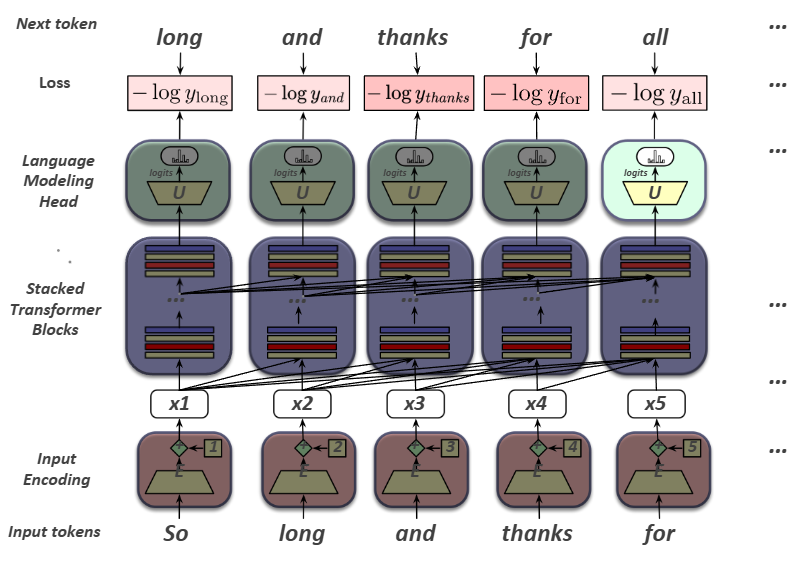
\includegraphics[width=0.9\linewidth]{pic/transformer_language_model_scheme.png}
                \caption{Transformer language model training scheme}
                \label{fig:transformer_language_model_scheme}
            \end{figure}
        \end{column}
        \begin{column}{0.4\textwidth}
            \[ \text{Total Batch Loss} = \frac{1}{T} \sum_{t=1}^{T} L_{CE} \]
        \end{column}
    \end{columns}
\end{frame}

%%%%%%%%%%%%%%%%%%%%%%%%%%%%%%%%%%%%%%%%%%%%%%%%%%
\section{Data Eng. and Fine-Tuning}

\begin{frame}{LLMs are mainly trained on the web}\justifying
    \begin{itemize}
        \item \textbf{Common Crawl:} Massive snapshots of the entire public web produced recursively by the non-profit Common Crawl organization, containing billions of raw HTML pages.
        \item \textbf{Colossal Clean Crawled Corpus (C4):} Authored by Raffel et al. (2020), this dataset contains 156 billion tokens of English text that have been rigorously filtered for quality.
        \item \textbf{What constitutes this data?} The bulk of the high-quality tokens are derived from patent text documents, Wikipedia dumps, and international news sites.
    \end{itemize}
\end{frame}

\begin{frame}{The Pile: an engineered pretraining corpus}\justifying
    A diverse, meticulously balanced 825 GiB open-source language modeling data set.
    \vspace{0.5cm}
    \begin{table}
        \centering
        \begin{tabular}{lll}
            \toprule
            \textbf{Academics} & \textbf{Web \& General} & \textbf{Books \& Dialog} \\
            \midrule
            PubMed Central & Pile-CC & Bibliotik \\
            ArXiv & OpenWebText2 & PG-19 \\
            FreeLaw & StackExchange & BookCorpus2 \\
            PhilPapers & Wikipedia & Ubuntu IRC / GitHub \\
            \bottomrule
        \end{tabular}
    \end{table}
\end{frame}

\begin{frame}{What does a model learn from pretraining?}\justifying
    The raw text ingested contains an enormous amount of human knowledge. Pre-training with billions of texts containing all this knowledge is what fundamentally gives language models their ability to execute so much logic.
    \begin{itemize}
        \item Contextual Logic: "There are canines everywhere! One dog in the front room, and two dogs."
        \item Semantic Scaling: "It wasn't just big it was enormous."
        \item Factual Retrieval: "The author of 'A Room of One's Own' is Virginia Woolf."
        \item Mathematical Truths: "The square root of 4 is 2."
    \end{itemize}
\end{frame}

\begin{frame}{Sociotechnical problems with scraping from the web}\justifying
    \begin{itemize}
        \item \textbf{Copyright Infringement:} A massive portion of the text in these datasets relies on copyrighted material. It is not clear if the fair use doctrine in the US allows for computational weight optimization. This remains a highly contentious open legal question.
        \item \textbf{Data Consent:} Website owners lack robust protocols to indicate they do not want their site crawled for AI training.
        \item \textbf{Privacy Violations:} Unfiltered websites can contain private IP addresses, social security metrics, and private phone numbers which the model may memorize.
    \end{itemize}
\end{frame}

\begin{frame}{Finetuning for Adaptation to New Domains}\justifying
    \textbf{What happens if we fundamentally need our LLM to work well on a highly specific domain it didn't encounter sufficiently in pretraining?}
    \begin{itemize}
        \item Perhaps some specific medical diagnostic phrasing or obscure legal contract domain?
        \item Or maybe a multilingual LM needs to see more data on a specific low-resource language that was statistically rare in the pretraining phase?
    \end{itemize}
\end{frame}

\begin{frame}{Finetuning as "continued pretraining"}\justifying
    \begin{itemize}
        \item The most direct approach is to further train all the billions of parameters of the model on the new specific data.
        \item We deploy the exact same method (next word prediction) and mathematical loss function (cross-entropy loss) as utilized for the original pretraining.
        \item We treat the operation as if the new specialized data were simply appended at the tail end of the massive pretraining data sequence.
        \item Hence, this process is frequently classified in literature as \textbf{continued pretraining}.
    \end{itemize}
\end{frame}

\begin{frame}{Finetuning}\justifying
    \begin{figure}
        \centering
        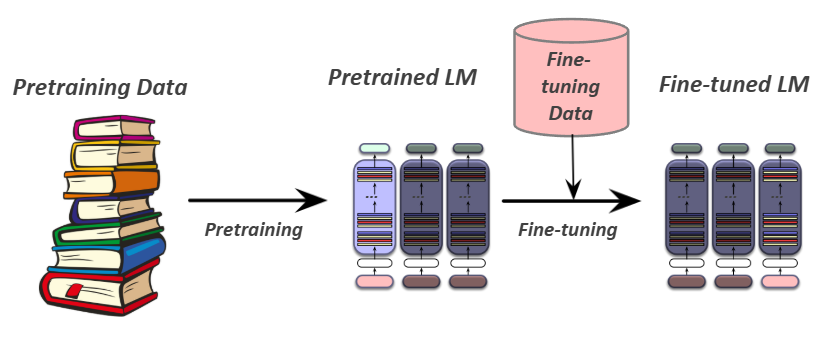
\includegraphics[width=\linewidth]{pic/finetuning.png}
        \caption{Finetuning flow}
        \label{fig:finetuning_flow}
    \end{figure}
\end{frame}

%%%%%%%%%%%%%%%%%%%%%%%%%%%%%%%%%%%%%%%%%%%%%%%%%%
\section{Evaluation, Scaling Laws, and Hard. Optim.}

\begin{frame}{Evaluating Large Language Models}
    \begin{center}
        \huge \textbf{Evaluating Large Language Models}\\
        \vspace{0.5cm}
        \Large Metrics and Scaling Infrastructure
    \end{center}
\end{frame}

\begin{frame}{Perplexity Metric}\justifying
    Just as for classical n-gram grammars, the industry uses Perplexity to mathematically measure how well the LM predicts unseen text distributions. \\
    \vspace{0.3cm}
    The perplexity of a model on an unseen test set is defined as the inverse probability that the model assigns to the test set, geometrically normalized by the test set length. \\
    \vspace{0.3cm}
    For a test sequence of $n$ tokens $w_{1:n}$, the perplexity is calculated as:
    \[ \text{Perplexity}(w_{1:n}) = P(w_{1:n})^{-\frac{1}{n}} \]
\end{frame}

\begin{frame}{Why perplexity instead of raw probability?}\justifying
    \begin{itemize}
        \item The raw probability metric depends entirely on the size of the test set; the probability asymptotically gets smaller the longer the text sequence runs.
        \item \textbf{The Superior Alternative:} A metric that operates per-word, rigorously normalized by the text length.
        \item Perplexity calculates the inverse probability of the test set, normalized by the total number of words. (This formulation derives directly from the cross-entropy rate in information theory).
        \item While probability operates on a tight range of $[0, 1]$, the perplexity range spans $[1, \infty]$.
        \item The higher the assigned probability of the word sequence, the lower the perplexity (indicating a vastly superior model).
    \end{itemize}
\end{frame}

\begin{frame}{Additional evaluation dimensions}\justifying
    \begin{itemize}
        \item \textbf{Size Constraints:} Large models require vast arrays of GPUs and thousands of hours to train, alongside immense VRAM memory just to store the parameters.
        \item \textbf{Energy Usage:} Evaluators must measure the physical kilowatt-hours (kWh) consumed or kilograms of CO2 emitted during training runs.
        \item \textbf{Fairness Benchmarks:} Specialized benchmarks are deployed to measure the generation of gendered and racial stereotypes, or the statistically decreased performance for language generated from or about marginalized socio-economic groups.
    \end{itemize}
\end{frame}

\begin{frame}{Scaling Laws}\justifying
    LLM empirical performance is strictly dependent upon:
    \begin{itemize}
        \item \textbf{Model size:} The absolute number of trainable parameters not counting the token embeddings.
        \item \textbf{Dataset size:} The raw volumetric amount of training data.
        \item \textbf{Compute:} The absolute amount of compute utilized (in FLOPs).
    \end{itemize}
    The performance of a large language model (measured by the loss) scales mathematically as a power-law with each of these three isolated variables:
    \[ L(N) = (N_c/N)^{\alpha_N} \]
    \[ L(D) = (D_c/D)^{\alpha_D} \]
    \[ L(C) = (C_c/C)^{\alpha_C} \]
\end{frame}

\begin{frame}{Number of non-embedding parameters N}\justifying
    We can mathematically estimate the total parameters via:
    \[ N \approx 2 d_{model} n_{layers} (2d_{attn} + d_{ff}) \]
    \[ \approx 12 n_{layers} d_{model}^2 \]
    Assuming standard dimensional ratios of $d_{attn} = d_{ff}/4 = d_{model}$. \\
    \vspace{0.5cm}
    Thus, calculating for the architecture of GPT-3, possessing $n=96$ layers and a massive dimensionality of $d=12288$, we determine:
    \[ 12 \times 96 \times 12288^2 \approx 175 \text{ billion parameters.} \]
\end{frame}

\begin{frame}{The KV Cache Bottleneck}\justifying
    During the pretraining phase, we can compute mathematical attention very efficiently in massive parallel batches. But this breaks down at inference! We are forced to generate the next tokens sequentially, one at a time.
    \begin{itemize}
        \item For every single new token $x$, we must multiply it by weight matrices $W_Q, W_K, W_V$ to generate a query, key, and values.
        \item But computing the attention score requires the key and value vectors for all the prior historical tokens $x_{<i}$, yielding an $O(N^2)$ computational disaster.
        \item \textbf{The Engineering Solution:} Permanently store the key and value vectors in GPU VRAM memory in the KV cache, and then simply grab them from the cache for $O(N)$ inference speed.
    \end{itemize}
\end{frame}

\begin{frame}{KV Cache Matrix Architecture}\justifying
    \begin{figure}
        \centering
        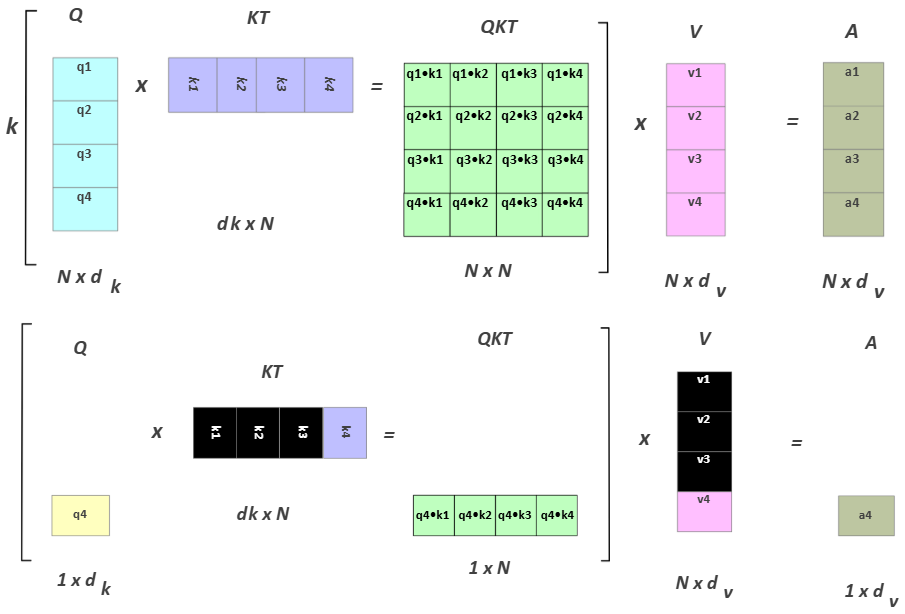
\includegraphics[width=0.6\linewidth]{pic/kv_cache.png}
        \caption{KV Chace representation}
        \label{fig:kv_cache_representation}
    \end{figure}
\end{frame}

\begin{frame}{Parameter-Efficient Finetuning (PEFT)}\justifying
    Adapting a generalized model to a highly specific new domain by continued full pretraining presents a massive infrastructure problem with huge LLMs:
    \begin{itemize}
        \item Enormous quantities of parameters to train, requiring massive optimizer memory overhead.
        \item Each pass of batch gradient descent must backpropagate entirely through many massive, deep layers.
        \item This is extraordinarily expensive in processing power, VRAM memory, and wall-clock time.
    \end{itemize}
    \textbf{The PEFT Paradigm:}
    \begin{itemize}
        \item Efficiently select an extremely small subset of parameters to update when finetuning.
        \item Freeze the vast majority of the parameters (don't alter them), and only mathematically update a few specialized parameters.
    \end{itemize}
\end{frame}

\begin{frame}{LORA (Low-Rank Adaptation) Theory}\justifying
    \begin{itemize}
        \item Standard Transformers consist of many dense matrix multiplication layers.
        \item Like the $W_Q, W_K, W_V, W_O$ layers utilized in the attention mechanism.
        \item Instead of updating these massive full-rank layers during finetuning iterations...
        \item We permanently freeze these base layers; and we mathematically update a low-rank approximation containing drastically fewer parameters.
    \end{itemize}
\end{frame}

\begin{frame}{LORA Mathematics}\justifying
    Consider a base weight matrix $W$ (shape $N \times d$) that theoretically needs to be updated during finetuning via gradient descent. Normally the updates form a dense matrix $\Delta W$ (shape $N \times d$). \\
    \vspace{0.3cm}
    In the LORA algorithm, we freeze $W$ and update instead a low-rank decomposition of $W$:
    \begin{itemize}
        \item Matrix $A$ possessing shape $N \times r$
        \item Matrix $B$ possessing shape $r \times d$
        \item Critically, $r$ (rank) is very small (like 1, 2, or 8)
    \end{itemize}
    We computationally replace $W + \Delta W$ with $W + BA$. \\
    Forward pass: instead of $h = xW$, we calculate:
    \[ h = xW + xAB \]
\end{frame}

\begin{frame}{LoRA}
    \begin{figure}
        \centering
        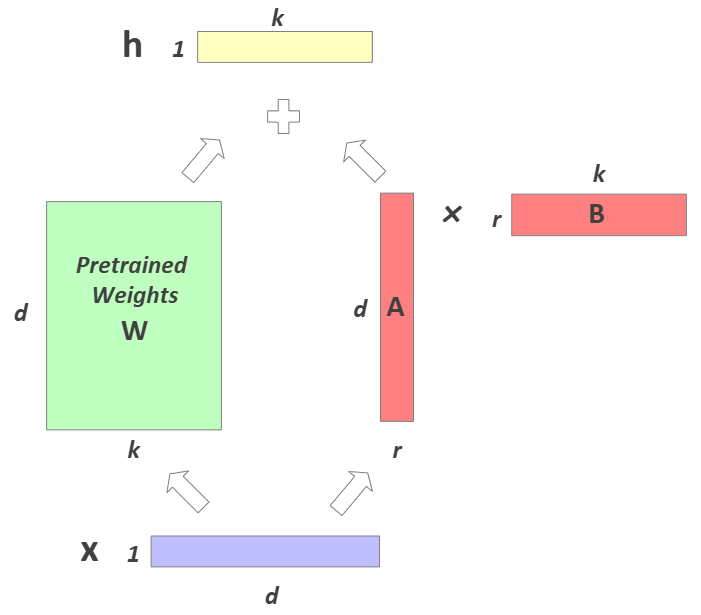
\includegraphics[width=0.5\linewidth]{pic/lora.png}
        \caption{LoRA representation}
        \label{fig:lora_representation}
    \end{figure}
\end{frame}

\begin{frame}{Full Fine-Tuning vs. LoRA Integration}\justifying
    \textbf{Full Fine-Tuning Profile:}
    \begin{itemize}
        \item Update all model parameters ($\approx 175B$)
        \item Storage Requirement: Huge
        \item Compute Required: High
        \item Processing Speed: Slow
    \end{itemize}
    \vspace{0.5cm}
    \textbf{LoRA (Low-Rank Adaptation) Profile:}
    \begin{itemize}
        \item Keep Pretrained Model Frozen. Add a Tiny LoRA Plugin in parallel.
        \item Small individual adapter generated per task ($\approx 17M$ params)
        \item Storage Requirement: Minimal
        \item Compute Required: Low
        \item Processing Speed: Fast
    \end{itemize}
\end{frame}

\begin{frame}{Full Fine-Tuning \& LoRA}
    \begin{figure}
        \centering
        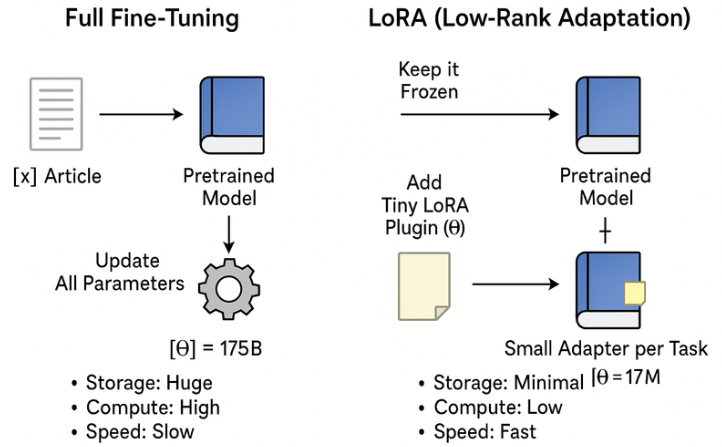
\includegraphics[width=0.7\linewidth]{pic/full_fine-tuning_vs_lora.png}
        \caption{Full Fine-Tuning \& LoRA flow}
        \label{fig:full_fine-tuning_LoRA_flow}
    \end{figure}
\end{frame}

\begin{frame}{Societal Harms of Large Language Models}\justifying
    \begin{itemize}
        \item \textbf{Hallucination}
        \item \textbf{Copyright Litigation}
        \item \textbf{Privacy Breaches}
        \item \textbf{Toxicity and Exploitation}
        \item \textbf{Political Misinformation}
    \end{itemize}
\end{frame}

\begin{frame}{Hallucination}
    Chatbots routinely 'hallucinate' fake corporate policies or non-existent facts. Individuals currently possess little protection or legal recourse when the technology autonomously creates and spreads falsehoods about them.
    \vspace{0.5cm}
    
    \begin{figure}[htbp]
      \centering
      \framebox{\parbox{0.6\textwidth}{\centering
        \vspace{1cm}
        \textbf{Space for Image} \\
        \small\textit{Insert the hallucination image from news here.}
        \vspace{1cm}
      }}
    \end{figure}
\end{frame}

\begin{frame}{Copyright Litigation}
    Authors and media conglomerates are actively suing corporations, claiming mass copyright infringement regarding the hundreds of thousands of novels and news articles utilized without permission during training.
    \vspace{0.5cm}
    
    \begin{figure}[htbp]
      \centering
      \framebox{\parbox{0.6\textwidth}{\centering
        \vspace{1cm}
        \textbf{Space for Image} \\
        \small\textit{Insert the copyright litigation image from news here.}
        \vspace{1cm}
      }}
    \end{figure}
\end{frame}

\begin{frame}{Privacy Breaches}
    The models have demonstrated the ability to leak private email addresses and phone numbers extracted from the training data.
    \vspace{0.5cm}
    
    \begin{figure}[htbp]
      \centering
      \framebox{\parbox{0.6\textwidth}{\centering
        \vspace{1cm}
        \textbf{Space for Image} \\
        \small\textit{Insert the privacy breaches image from news here.}
        \vspace{1cm}
      }}
    \end{figure}
\end{frame}

\begin{frame}{Toxicity and Exploitation}
    Chatbots threaten users, while cleaning up the training data exacts a horrific psychological toll on human contractors forced to read descriptions of violence and abuse.
    \vspace{0.5cm}
    
    \begin{figure}[htbp]
      \centering
      \framebox{\parbox{0.6\textwidth}{\centering
        \vspace{1cm}
        \textbf{Space for Image} \\
        \small\textit{Insert the toxicity and exploitation image from news here.}
        \vspace{1cm}
      }}
    \end{figure}
\end{frame}

\begin{frame}{Political Misinformation}
    The generation of highly persuasive false and misleading information regarding global elections.
    \vspace{0.5cm}
    
    \begin{figure}[htbp]
      \centering
      \framebox{\parbox{0.6\textwidth}{\centering
        \vspace{1cm}
        \textbf{Space for Image} \\
        \small\textit{Insert the political misinformation image from news here.}
        \vspace{1cm}
      }}
    \end{figure}
\end{frame}

%%%%%%%%%%%%%%%%%%%%%%%%%%%%%%%%%%%%%%%%%%%%%%%%%%
\section{References}

\begin{frame}[allowframebreaks]{References}\justifying
    \begin{thebibliography}{99}
    \scriptsize
    
    \bibitem{anthropic2025} Anthropic. 2025. Release notes: System prompts.
    \bibitem{bellegarda1997} Bellegarda, J. R. 1997. A latent semantic analysis framework for large-span language modeling. EUROSPEECH.
    \bibitem{bengio2000} Bengio, Y., R. Ducharme, and P. Vincent. 2000. A neural probabilistic language model. NeurIPS.
    \bibitem{bengio2003} Bengio, Y., R. Ducharme, P. Vincent, and C. Jauvin. 2003. A neural probabilistic language model. JMLR.
    \bibitem{bengio2006} Bengio, Y., et al. 2006. Neural probabilistic language models. In Innovations in Machine Learning. Springer.
    \bibitem{bickmore2018} Bickmore, T. W., et al. 2018. Patient and consumer safety risks when using conversational assistants... Journal of Medical Internet Research.
    \bibitem{blodgett2020} Blodgett, S. L., et al. 2020. Language (technology) is power: A critical survey of “bias” in NLP. ACL.
    \bibitem{bommasani2021} Bommasani, R., et al. 2021. On the opportunities and risks of foundation models. ArXiv.
    \bibitem{brown2020} Brown, T., et al. 2020. Language models are few-shot learners. NeurIPS.
    \bibitem{carlini2021} Carlini, N., et al. 2021. Extracting training data from large language models. USENIX Security 21.
    \bibitem{cheng2023} Cheng, M., E. Durmus, and D. Jurafsky. 2023. Marked personas: Using natural language prompts to measure stereotypes... ACL.
    \bibitem{cheng2025} Cheng, M., et al. 2025. Sycophantic ai decreases prosocial intentions and promotes dependence. ArXiv.
    \bibitem{coccaro1998} Coccaro, N. and D. Jurafsky. 1998. Towards better integration of semantic predictors in statistical language modeling. ICSLP.
    \bibitem{dai2015} Dai, A. M. and Q. V. Le. 2015. Semi-supervised sequence learning. NeurIPS.
    \bibitem{deerwester1988} Deerwester, S. C., et al. 1988. Computer information retrieval using latent semantic structure: US Patent 4,839,853.
    \bibitem{devlin2019} Devlin, J., et al. 2019. BERT: Pre-training of deep bidirectional transformers for language understanding. NAACL HLT.
    \bibitem{dinan2021} Dinan, E., et al. 2021. Anticipating safety issues in e2e conversational ai: Framework and tooling. ArXiv.
    \bibitem{dinan2020} Dinan, E., et al. 2020. Queens are powerful too: Mitigating gender bias in dialogue generation. EMNLP.
    \bibitem{dodge2019} Dodge, J., et al. 2019. Show your work: Improved reporting of experimental results. EMNLP.
    \bibitem{dodge2021} Dodge, J., et al. 2021. Documenting large webtext corpora. EMNLP.
    \bibitem{ethayarajh2020} Ethayarajh, K. and D. Jurafsky. 2020. Utility is in the eye of the user: A critique of NLP leaderboards. EMNLP.
    \bibitem{friedman2019} Friedman, B. and D. G. Hendry. 2019. Value Sensitive Design: Shaping Technology with Moral Imagination. MIT Press.
    \bibitem{friedman2017} Friedman, B., et al. 2017. A survey of value sensitive design methods. Foundations and Trends in Human-Computer Interaction.
    \bibitem{gao2020} Gao, L., et al. 2020. The Pile: An 800GB dataset of diverse text for language modeling. ArXiv.
    \bibitem{gehman2020} Gehman, S., et al. 2020. RealToxicityPrompts: Evaluating neural toxic degeneration in language models. Findings of EMNLP.
    \bibitem{gururangan2020} Gururangan, S., et al. 2020. Don’t stop pretraining: Adapt language models to domains and tasks. ACL.
    \bibitem{hashimoto2018} Hashimoto, T., et al. 2018. Fairness without demographics in repeated loss minimization. ICML.
    \bibitem{heafield2011} Heafield, K. 2011. KenLM: Faster and smaller language model queries. WMT.
    \bibitem{henderson2020} Henderson, P., et al. 2020. Towards the systematic reporting of the energy and carbon footprints of machine learning. JMLR.
    \bibitem{henderson2023} Henderson, P., et al. 2023. Foundation models and fair use. JMLR.
    \bibitem{henderson2017} Henderson, P., et al. 2017. Ethical challenges in data-driven dialogue systems. AAAI/ACM.
    \bibitem{hofmann2024} Hofmann, V., et al. 2024. Ai generates covertly racist decisions about people based on their dialect. Nature.
    \bibitem{ischen2019} Ischen, C., et al. 2019. Privacy concerns in chatbot interactions. International Workshop.
    \bibitem{jelinek1975} Jelinek, F., et al. 1975. Design of a linguistic statistical decoder for the recognition of continuous speech. IEEE.
    \bibitem{khattab2024} Khattab, O., et al. 2024. DSPy: Compiling declarative language model calls into self-improving pipelines. ICLR.
    \bibitem{kiela2021} Kiela, D., et al. 2021. Dynabench: Rethinking benchmarking in NLP. NAACL HLT.
    \bibitem{landauer1997} Landauer, T. K., et al. 1997. How well can passage meaning be derived without using word order? COGSCI.
    \bibitem{liang2023} Liang, P., et al. 2023. Holistic evaluation of language models. Transactions on Machine Learning Research.
    \bibitem{liu2020} Liu, H., et al. 2020. Does gender matter? Towards fairness in dialogue systems. COLING.
    \bibitem{llama2024} Llama Team. 2024. The llama 3 herd of models.
    \bibitem{longpre2024a} Longpre, S., et al. 2024a. Consent in crisis: The rapid decline of the ai data commons. ArXiv.
    \bibitem{longpre2024b} Longpre, S., et al. 2024b. A pretrainer’s guide to training data. NAACL HLT.
    \bibitem{mcguffie2020} McGuffie, K. and A. Newhouse. 2020. The radicalization risks of GPT-3 and advanced neural language models. ArXiv.
    \bibitem{mikolov2013a} Mikolov, T., et al. 2013a. Efficient estimation of word representations in vector space. ICLR.
    \bibitem{mikolov2010} Mikolov, T., et al. 2010. Recurrent neural network based language model. INTERSPEECH.
    \bibitem{mikolov2011} Mikolov, T., et al. 2011. Extensions of recurrent neural network language model. ICASSP.
    \bibitem{mikolov2013b} Mikolov, T., et al. 2013b. Distributed representations of words and phrases and their compositionality. NeurIPS.
    \bibitem{miller1950} Miller, G. A. and J. A. Selfridge. 1950. Verbal context and the recall of meaningful material.
    \bibitem{min2022} Min, S., et al. 2022. Rethinking the role of demonstrations: What makes in-context learning work? EMNLP.
    \bibitem{nadeem2021} Nadeem, M., A. Bethke, and S. Reddy. 2021. StereoSet: Measuring stereotypical bias... ACL.
    \bibitem{neff2016} Neff, G. and P. Nagy. 2016. Talking to bots: Symbiotic agency and the case of Tay.
    \bibitem{parrish2022} Parrish, A., et al. 2022. BBQ: A hand-built bias benchmark for question answering. Findings of ACL.
    \bibitem{peters2018} Peters, M., et al. 2018. Deep contextualized word representations. NAACL HLT.
    \bibitem{radford2019} Radford, A., et al. 2019. Language models are unsupervised multitask learners. OpenAI.
    \bibitem{raffel2020} Raffel, C., et al. 2020. Exploring the limits of transfer learning with a unified text-to-text transformer. JMLR.
    \bibitem{rawls2001} Rawls, J. 2001. Justice as fairness: A restatement. Harvard University Press.
    \bibitem{reeves1996} Reeves, B. and C. Nass. 1996. The Media Equation. Cambridge University Press.
    \bibitem{rosenfeld1992} Rosenfeld, R. 1992. Adaptive Statistical Language Modeling: A Maximum Entropy Approach.
    \bibitem{rosenfeld1996} Rosenfeld, R. 1996. A maximum entropy approach to adaptive statistical language modeling.
    \bibitem{sagawa2020} Sagawa, S., et al. 2020. Distributionally robust neural networks for group shifts. ICLR.
    \bibitem{shannon1948} Shannon, C. E. 1948. A mathematical theory of communication.
    \bibitem{sheng2019} Sheng, E., et al. 2019. The woman worked as a babysitter: On biases in language generation. EMNLP.
    \bibitem{soldaini2024} Soldaini, L., et al. 2024. Dolma: An open corpus of three trillion tokens for language model pretraining research. ArXiv.
    \bibitem{stolcke2002} Stolcke, A. 2002. SRILM – an extensible language modeling toolkit. ICSLP.
    \bibitem{strubell2019} Strubell, E., A. Ganesh, and A. McCallum. 2019. Energy and policy considerations for deep learning in NLP. ACL.
    \bibitem{vaswani2017} Vaswani, A., et al. 2017. Attention is all you need. NeurIPS.
    \bibitem{webson2022} Webson, A. and E. Pavlick. 2022. Do prompt-based models really understand the meaning of their prompts? NAACL HLT.
    \bibitem{weizenbaum1966} Weizenbaum, J. 1966. ELIZA. CACM.
    \bibitem{wolf2017} Wolf, M. J., et al. 2017. Why we should have seen that coming: Comments on Microsoft’s Tay. The ORBIT Journal.
    \bibitem{xu2021} Xu, A., et al. 2021. Detoxifying language models risks marginalizing minority voices. NAACL HLT.
    \bibitem{xu2020} Xu, J., et al. 2020. Recipes for safety in open-domain chatbots. ArXiv.
    \bibitem{zaosanders2025} Zao-Sanders, M. 2025. How People Are Really Using Gen AI in 2025.
    \bibitem{zhang2025} Zhang, A. K., et al. 2025. Language model developers should report train-test overlap. ICML.
    
    \end{thebibliography}
\end{frame}

%%%%%%%%%%%%%%%%%%%%%%%%%%%%%%%%%%%%%%%%%%%%%%%%%%
\begin{frame}
    \begin{center}
        \Large \textbf{THANK YOU SO MUCH}
    \end{center}
\end{frame}
%%%%%%%%%%%%%%%%%%%%%%%%%%%%%%%%%%%%%%%%%%%%%%%%%%
\end{document}